% engl. natural numbers, counting numbers
% ruots. naturliga tal

% Luonnollisia lukuja käytetään kolmeen eri tarkoitukseen:
% Lukumäärien ilmoittamiseen (kardinaaliluvut)
% Järjestyksen ilmoittamiseen (ordinaaliluvut)
% Indeksointiin ja asioiden nimeämiseen

% FIXME: tähän voisi lisätä lyhyen, selkeän johdannon muuttujien käytön etuihin

% === SIISTITTÄVÄ PÄTKÄ ALKAA ===

Luonnollisille luvuille $m$ ja $n$ on määritelty yhteenlasku $m + n$, esimerkiksi $5 + 3 = 8$.

Luonnollisten lukujen $m$ ja $n$ kertolasku määritellään peräkkäisinä yhteenlaskuina
\laatikko{ \[m \cdot n = \underbrace{m + m + \ldots + m}_{n\text{ kpl}} = \underbrace{n + n + \ldots + n}_{m\text{ kpl}}.\] }

Nollalla kertomisen ajatellaan olevan ''tyhjä yhteenlasku'' eli nolla:
\laatikko{ \[0 \cdot m = 0\] }

Luonnollisten lukujen $m$ ja $n$ erotus määritellään yhteenlaskun avulla:
$m-n$ on luku $k$, jolle $k + n = m$. Kahden luonnollisen luvun erotus
ei kuitenkaan aina ole luonnollinen luku, esimerkkinä $3 - 5$.
Ratkaisemme ongelman määrittelemällä kullekin luonnolliselle
luvulle vastaluvun.

\laatikko{ Jokaisella luvulla $n$ on vastaluku $-n$, jolle pätee $n+(-n)=0$. }

Luonnolliset luvut ja niiden vastaluvut muodostavat yhdessä kokonaislukujen joukon

\[\zz = \{\ldots, -2, -1, 0, 1, 2, \ldots\},\] jota voidaan havainnollistaa \termi{lukusuora}{lukusuoran} avulla

\begin{kuva}
	lukusuora.pohja(-4,4,12)
	lukusuora.piste(-3, "$-3$")
	lukusuora.piste(-2,"$-2$")
	lukusuora.piste(-1,"$-1$")
	lukusuora.piste(0,"$0$")
	lukusuora.piste(1,"$1$")
	lukusuora.piste(2,"$2$")
	lukusuora.piste(3,"$3$")
\end{kuva}

%\begin{center}
%\begin{lukusuora}{-4}{4}{10}
%\lukusuorapiste{-3}{}
%\lukusuorapiste{-2}{}
%\lukusuorapiste{-1}{}
%\lukusuorapiste{0}{}
%\lukusuorapiste{1}{}
%\lukusuorapiste{2}{}
%\lukusuorapiste{3}{}
%\lukusuoraalanimi{-3}{$-3$}
%\lukusuoraalanimi{-2}{$-2$}
%\lukusuoraalanimi{-1}{$-1$}
%\lukusuoraalanimi{0}{$0$}
%\lukusuoraalanimi{1}{$1$}
%\lukusuoraalanimi{2}{$2$}
%\lukusuoraalanimi{3}{$3$}
%
%\end{lukusuora}
%\end{center}


Kun käytämme kokonaislukuja, voidaan kahden luvun erotus määritellä
yhteenlaskun ja vastaluvun avulla yksinkertaisesti:

\laatikko{
\[m-n = m+(-n)\]
}

    Esimerkiksi luvun $2$ vastalukua merkitään $-2$, ja sille pätee $2+(-2)=0$. Vastaavasti luvun $-2$ vastaluku on sellainen luku, joka laskettuna yhteen luvun $-2$ kanssa antaa luvun $0$. Tämä on tietysti $2$, koska $-2+2=0$. Näin voidaan huomata, että $-(-2)=2$.
    
\laatikko{$$-(-a)=a$$}

\subsection*{Yhteen- ja vähennyslasku}

    Kysymys: Mitä saadaan, kun luvusta $5$ vähennetään luku $-8$?
    
    Negatiivisten ja positiivisten lukujen yhteen- ja vähennyslaskut voidaan helposti tulkita lukusuoran avulla.
    
    % tässä on vähän kyseenalaista käyttää sekaisin sanallista ja numeerista esitystä
    
    $5+8$ ''viiteen lisätään kahdeksan''
\begin{center}
\begin{kuva}
	lukusuora.pohja(-4,14,12,n=2)
	with vari("red"):
		lukusuora.vali(0,5,i=1)
		lukusuora.vali(8,13,i=2)
	with vari("blue"): lukusuora.vali(0,8,i=2)
	lukusuora.piste(0,"$0$")
	lukusuora.piste(5,"$5$",1)
	lukusuora.piste(8,"$8$",2)
	lukusuora.piste(13,"$13$",2)
\end{kuva}
%      \begin{lukusuora}{-1}{14}{14}
%        %\lukusuoranuolialas{5}{13}
%        %\lukusuoranuolialas{0}{8}
%        {\color{red} \lukusuoravaliss{0}{5}{$0$}{$5$}}
%        \lukusuorauusi
%        {\color{red} \lukusuoravaliss{8}{13}{$8$}{${\color{black}13}$}}
%        {\color{blue} \lukusuoravaliss{0}{8}{$0$}{$8$}}
%       \end{lukusuora}
       ${\color{red}5}+{\color{blue}8}=13$
\end{center}
    
    $5+(+8)$ ''viiteen lisätään plus kahdeksan''
    
    $+8$ tarkoittaa samaa kuin $8$. '$+$'-merkkiä käytetään luvun edessä silloin, kun halutaan korostaa, että kyseessä on nimenomaan positiivinen luku.
    
%säädetään kuva vähän irti tuosta edeltävästä tektistä
%\vspace{0.3cm}     
    
\begin{center}
\begin{kuva}
	lukusuora.pohja(-4,14,12,n=2)
	with vari("red"):
		lukusuora.vali(0,5,i=1)
		lukusuora.vali(8,13,i=2)
	with vari("blue"): lukusuora.vali(0,8,i=2)
	lukusuora.piste(0,"$0$")
	lukusuora.piste(5,"$5$",1)
	lukusuora.piste(8,"$8$",2)
	lukusuora.piste(13,"$13$",2)
\end{kuva}
%          \begin{lukusuora}{-1}{14}{14}
%        {\color{red} \lukusuoravaliss{0}{5}{$0$}{$5$}}
%        \lukusuorauusi
%        {\color{red} \lukusuoravaliss{8}{13}{$8$}{${\color{black}13}$}}
%        {\color{blue} \lukusuoravaliss{0}{8}{$0$}{$8$}}
%       \end{lukusuora}
       ${\color{red}5}+({\color{blue}+8})=13$
\end{center}
    
    $5-(+8)$ ''viidestä vähennetään $+8$''
    
    Tämä tarkoittaa samaa kuin $5-8$. Lukusuoralla siis liikutaan 8 pykälää taaksepäin.

%säädetään kuva vähän irti tuosta edeltävästä tektistä
\vspace{0.3cm}     
    
\begin{center}
\begin{kuva}
	lukusuora.pohja(-4,14,12,n=2)
	with vari("red"):
		lukusuora.vali(0,5,i=2)
	with vari("blue"): lukusuora.vali(-3,5,i=1)
	lukusuora.piste(0,"$0$",2)
	lukusuora.piste(5,"$5$")
	lukusuora.piste(-3,"$-3$",1)
\end{kuva}
%              \begin{lukusuora}{-4}{8}{14}
%        {\color{blue} \lukusuoravaliss{-3}{5}{\color{black}$-3$}{$5$}}
%        \lukusuorauusi
%%        {\color{red} \lukusuoravaliss{8}{13}{$8$}{${\color{black}13}$}}
%        {\color{red} \lukusuoravaliss{0}{5}{$0$}{$5$}}
%       \end{lukusuora}
       ${\color{red}5}-({\color{blue}+8})=-3$
\end{center}


%lukiolaiset pitivät näitä epäselvinä kuvina
    
Mitä tapahtuu, kun lisätään negatiivinen luku? Kun lukuun lisätään $1$, se kasvaa yhdellä. Kun lukuun lisätään $0$, se ei kasva lainkaan. Kun lukuun lisätään negatiivinen luku, esimerkiksi $-1$, on luonnollista ajatella, että se pienenee. Tällä logiikalla negatiivisen luvun lisäämisen pitäisi siis pienentää alkuperäistä lukua. Juuri näin vähennyslasku määritellään: $5+(-8)$ on yhtä suuri kuin $5-8$.
    
\vspace{0.3cm}     
\begin{center}
\begin{kuva}
	lukusuora.pohja(-4,14,12,n=2)
	with vari("red"):
		lukusuora.vali(0,5,i=2)
	with vari("blue"): lukusuora.vali(-3,5,i=1)
	lukusuora.piste(0,"$0$",2)
	lukusuora.piste(5,"$5$")
	lukusuora.piste(-3,"$-3$",1)
\end{kuva}
%                 \begin{lukusuora}{-4}{8}{14}
%        {\color{blue} \lukusuoravaliss{-3}{5}{\color{black}$-3$}{$5$}}
%        \lukusuorauusi
%%        {\color{red} \lukusuoravaliss{8}{13}{$8$}{${\color{black}13}$}}
%        {\color{red} \lukusuoravaliss{0}{5}{$0$}{$5$}}
%       \end{lukusuora}
       ${\color{red}5}+({\color{blue}-8})=-3$
\end{center}
    
    
    $5-(-8)$ ''viidestä vähennetään miinus kahdeksan''
    
    Negatiivisen luvun lisääminen on vastakohta positiivisen luvun lisäämiselle. Tällöin on luonnollista, että negatiivisen luvun vähentäminen on vastakohta positiivisen luvun vähentämiselle. Koska positiivisen luvun vähentäminen pienentää lukua, pitäisi negatiivisen luvun vähentämisen kasvattaa lukua. Lasku $5-(-8)$ tarkoittaa siis samaa kuin $5+8$.
\vspace{0.3cm}     
        
\begin{center}
\begin{kuva}
	lukusuora.pohja(-4,14,12,n=2)
	with vari("red"):
		lukusuora.vali(0,5,i=1)
		lukusuora.vali(8,13,i=2)
	with vari("blue"): lukusuora.vali(0,8,i=2)
	lukusuora.piste(0,"$0$")
	lukusuora.piste(5,"$5$",1)
	lukusuora.piste(8,"$8$",2)
	lukusuora.piste(13,"$13$",2)
\end{kuva}
%    \begin{lukusuora}{-1}{14}{14}
%        {\color{red} \lukusuoravaliss{0}{5}{$0$}{$5$}}
%        \lukusuorauusi
%        {\color{red} \lukusuoravaliss{8}{13}{$8$}{${\color{black}13}$}}
%        {\color{blue} \lukusuoravaliss{0}{8}{$0$}{$8$}}
%       \end{lukusuora}
       ${\color{red}5}-({\color{blue}-8})=13$
\end{center}


\laatikko{
Yhteen- ja vähennyslaskun merkkisäännöt

\begin{alakohdat}
\alakohta{$a+(+b)=a+b$}
\alakohta{$a+(-b)=a-b$}
\alakohta{$a-(+b)=a-b$}
\alakohta{$a-(-b)=a+b$}
\end{alakohdat}
}

%Koska $+b-b=0$, yhteen- ja vähennyslasku kumoavat toisensa, eli
%
%\begin{itemize}
%\alakohta{$a+b-b=a$
%\alakohta{$a-b+b=a$
%\end{itemize}



\subsection*{Kertolasku}

    Samaan logiikkaan perustuen on sovittu myös merkkisäännöt positiivisten ja negatiivisten lukujen kertolaskuissa. Kun negatiivinen ja positiivinen luku kerrotaan keskenään, saadaan negatiivinen luku, mutta kun kaksi negatiivista lukua kerrotaan keskenään, saadaan positiivinen luku.

    $3 \cdot 4$ ''kolme kappaletta nelosia''
    
\begin{center}
\begin{kuva}
	lukusuora.pohja(-14,14,12)
	vari("red")
	lukusuora.vali(0,4)
	lukusuora.vali(4,8)
	lukusuora.vali(8,12)
	vari("black")
	lukusuora.piste(0,"$0$")
	lukusuora.piste(4,"$4$")
	lukusuora.piste(8,"$8$")
	lukusuora.piste(12,"$12$")
\end{kuva}
%    \begin{lukusuora}{-1}{14}{14}
%	\color{red} \lukusuoravaliss{0}{4}{$0$}{$4$}
%	\color{red} \lukusuoravaliss{4}{8}{$4$}{$8$}
%	\color{red} \lukusuoravaliss{8}{12}{$8$}{$12$}
%
%      \end{lukusuora}
      $3\cdot {\color{red}4}=12$
\end{center}
    
    $3 \cdot (-4)$ ''kolme kappaletta miinus-nelosia''
    
    
\begin{center}
\begin{kuva}
	lukusuora.pohja(-14,14,12)
	vari("red")
	lukusuora.vali(-4,0)
	lukusuora.vali(-8,-4)
	lukusuora.vali(-12,-8)
	vari("black")
	lukusuora.piste(0,"$0$")
	lukusuora.piste(-4,"$-4$")
	lukusuora.piste(-8,"$-8$")
	lukusuora.piste(-12,"$-12$")
\end{kuva}
%    \begin{lukusuora}{-13}{2}{14}
%	\color{red} \lukusuoravaliss{-12}{-8}{$-12$}{$-8$}
%	\color{red} \lukusuoravaliss{-8}{-4}{$-8$}{$-4$}
%	\color{red} \lukusuoravaliss{-4}{0}{$-4$}{$0$}
%
%      \end{lukusuora}
      $3\cdot ({\color{red}-4})=-12$
\end{center}
    
    $-3 \cdot 4$ ''miinus-kolme nelinkertaistetaan''
    
\begin{center}
\begin{kuva}
	lukusuora.pohja(-14,14,12)
	vari("blue")
	lukusuora.vali(-3,0)
	lukusuora.vali(-6,-3)
	lukusuora.vali(-9,-6)
	lukusuora.vali(-12,-9)
	vari("black")
	lukusuora.piste(0,"$0$")
	lukusuora.piste(-3,"$-3$")
	lukusuora.piste(-6,"$-6$")
	lukusuora.piste(-9,"$-9$")
	lukusuora.piste(-12,"$-12$")
\end{kuva}
%    \begin{lukusuora}{-13}{2}{14}
%	\color{red} \lukusuoravaliss{-12}{-9}{$-12$}{$-9$}
%	\color{red} \lukusuoravaliss{-9}{-6}{$-9$}{$-6$}
%	\color{red} \lukusuoravaliss{-6}{-3}{$-6$}{$-3$}
%	\color{red} \lukusuoravaliss{-3}{0}{$-3$}{$0$}
%
%      \end{lukusuora}
      ${\color{blue}-3}\cdot 4=-12$
\end{center}
    
    $-3 \cdot (-4)$ ''miinus-kolme miinus-nelinkertaistetaan''
    
\begin{center}
\begin{kuva}
	lukusuora.pohja(-14,14,12)
	vari("blue")
	lukusuora.vali(0,3)
	lukusuora.vali(3,6)
	lukusuora.vali(6,9)
	lukusuora.vali(9,12)
	vari("black")
	lukusuora.piste(0,"$0$")
	lukusuora.piste(3,"$3$")
	lukusuora.piste(6,"$6$")
	lukusuora.piste(9,"$9$")
	lukusuora.piste(12,"$12$")
\end{kuva}
%    \begin{lukusuora}{-1}{14}{14}
%	\color{red} \lukusuoravaliss{12}{9}{$12$}{$9$}
%	\color{red} \lukusuoravaliss{9}{6}{$9$}{$6$}
%	\color{red} \lukusuoravaliss{6}{3}{$6$}{$3$}
%	\color{red} \lukusuoravaliss{3}{0}{$3$}{$0$}
%
%      \end{lukusuora}
      ${\color{blue}-3}\cdot (-4)=12$
\end{center}

\subsection*{Jakolasku}

        Kun ensin kerrotaan jollain ja sitten jaetaan samalla luvulla, päädytään takaisin samaan, mistä lähdettiin.  Jakolaskujen merkkisäännöt on sovittu niin, että tämä ominaisuus säilyy. Ne ovat siis samat kuin kertolaskujen merkkisäännöt.
    
    Esimerkiksi haluamme, että $(-12):(-3)\cdot (-3)=-12$. Nyt voimme kysyä, mitä laskun $(-12):(-3)$ tulokseksi pitäisi tulla, jotta jakolasku ja kertolasku säilyvät toisilleen käänteisinä, eli mikä luku kerrottuna luvulla $-3$ on $-12$. Kertolaskun merkkisäännöistä nähdään helposti, että tämän luvun täytyy olla $+4$ eli $4$. Niinpä on sovittu, että $(-12):(-3)=12:3=4$.

\laatikko{
Kerto- ja jakolaskun merkkisäännöt
\begin{alakohdat}
\alakohta{$a\cdot (-b)=(-a)\cdot b=-(ab)$}
\alakohta{$(-a)\cdot (-b)=a\cdot b=ab$}
\alakohta{$(-a):b=a:(-b)=-\dfrac{a}{b}$}
\alakohta{$(-a):(-b)=a: b=\dfrac{a}{b}$}
\end{alakohdat}
}

\laatikko{
Kerto- ja jakolasku kumoavat toisensa
\begin{alakohdat}
\alakohta{$a\cdot b:b=a$}
\alakohta{$a:b\cdot b=a$}
\end{alakohdat}
}

\subsection*{Lausekkeiden sieventäminen}

Matemaattisia ongelmia ratkaistaessa kannattaa usein etsiä vaihtoehtoisia tapoja jonkin laskutoimituksen, lausekkeen tai luvun ilmaisemiseksi. Tällöin usein korvataan esimerkiksi jokin laskutoimitus toisella laskutoimituksella, josta tulee sama tulos. Näin lauseke saadaan sellaiseen muotoon, jonka avulla ratkaisussa päästään eteenpäin. Kun merkitsemme monimutkaisen lausekkeen lyhyemmin, sitä kutsutaan \termi{sieventäminen}{sieventämiseksi}. Sieventäminen on ikään kuin sotkuisen kaavan siistimistä selkeämmäksi.

Matematiikassa on tapana ajatella niin, että saman luvun voi kirjoittaa monella eri tavalla. Esimerkiksi merkinnät \begin{align*}
                & 42 \\ & -(-42) \\ & 6 \cdot 7 \\ & (50-29) \cdot 2                                                                                                      
                                                                                                                 \end{align*}
tarkoittavat kaikki samaa lukua. Niinpä missä tahansa lausekkeessa voi luvun $42$ paikalle kirjoittaa merkinnän $(50-29)\cdot 2$, sillä ne tarkoittavat samaa lukua. Tähän lukuun on koottu sääntöjä, joiden avulla laskutoimituksia voi vaihtaa niin, että lopputulos ei muutu.

\laatikko{
Yhteenlaskut voi laskea missä järjestyksessä tahansa

\begin{tabular}{ll}
  $a+b=b+a$\qquad\qquad&(vaihdantalaki)\\
  \\
  $a+(b+c)=(a+b)+c=a+b+c$\qquad\qquad&(liitäntälaki)
\end{tabular} 
}

Esimerkiksi laskemalla voidaan tarkistaa, että $5+7=7+5$ ja että $(2+3)+5=2+(3+5)$.

Nämä säännöt voidaan yhdistää yleiseksi säännöksi, jonka mukaan yhteenlaskun sisällä laskujärjestystä voi vaihtaa miten tahansa.

Tämä sääntö voidaan yleistää koskemaan myös vähennyslaskua, kun muistetaan, että vähennyslasku tarkoittaa oikeastaan vastaluvun lisäämistä. $5-8$ tarkoittaa siis samaa kuin $5+(-8)$, joka voidaan nyt kirjoittaa yhteenlaskun vaihdantalain perusteella muotoon $(-8)+5$ eli $-8+5$ ilman, että laskun lopputulos muuttuu. Tästä seuraa seuraava sääntö:

\laatikko{
Pelkästään yhteen- ja vähennyslaskua sisältävässä lausekkeessa laskujärjestystä voi vaihtaa vapaasti, kun ajattelee miinusmerkin kuuluvan sitä seuraavaan lukuun ja liikkuvan sen mukana.
}

\begin{esimerkki} 
$5-8+7-2=5+(-8)+7+(-2)=(-2)+(-8)+5+7=-2-8+5+7$ 
\end{esimerkki}

Vastaavat säännöt pätevät kerto- ja jakolaskulle samoista syistä.

\laatikko{
Kertolaskut voi laskea missä järjestyksessä tahansa

\begin{tabular}{ll}
  $a\cdot b=b\cdot a$\qquad\qquad&(vaihdantalaki)\\
  \\
  $a\cdot (b\cdot c)=(a\cdot b)\cdot c=a\cdot b\cdot c$\qquad\qquad&(liitäntälaki)
\end{tabular} 
}



\begin{esimerkki}

$5 \cdot 6 = 6 \cdot 5$
 
 $2 \cdot (1+2) = 2 \cdot 1 + 2 \cdot 2$
\end{esimerkki} 

%$2 \cdot (1+2) = 2 \cdot 1 + 2 \cdot 2$

\laatikko{
Pelkästään kerto- ja jakolaskua sisältävässä lausekkeessa laskujärjestystä voi vaihtaa vapaasti, kun ajattelee jakolaskun käänteisluvulla kertomisena.
}

\begin{esimerkki}
$5:8\cdot 7:2=5\cdot\frac18\cdot 7\cdot\frac12=7\cdot \frac12\cdot\frac18\cdot 5=7:2:8\cdot 5$
\end{esimerkki} 

Lisäksi yhteen- ja kertolaskua sisältävällä lausekkeelle pätee seuraava erittäin tärkeä sääntö:

\laatikko{
$a(b+c)=ab+ac$\qquad\qquad(osittelulaki)

Vasemmalta oikealle luettaessa puhutaan sulkujen avaamisesta. Oikealta vasemmalle päin mentäessä puhutaan \termi{yhteinen tekijä}{yhteisen tekijän ottamisesta}.
}

Aikaisemmin mainittujen laskulakien perusteella osittelulaki voidaan yhdistää koskemaan myös toisin päin olevaa kertolaskun ja yhteenlaskun yhdistelmää, useamman luvun yhteenlaskua, vähennyslaskua ja jakolaskua:

\begin{align*}
&(b+c)a = a(b+c) = ab+ac = ba+ca \text{ (Sovellettu vaihdantalakia)} \\
&a(b+c+d) = a((b+c)+d) = a(b+c)+ad = ab+ac+ad \text{ (Sovellettu liitäntälakia)} \\
&a(b-c) = a(b+(-c))=ab+a\cdot(-c)=ab-ac \text{ (Sovellettu vähennyslaskun määritelmää vastaluvun avulla)} \\
&(b+c):a = (b+c)\cdot\dfrac1a = b\cdot\dfrac1a+c\cdot\dfrac1a = b:a+c:a \text{ (Sovellettu jakolaskun ilmaisemista käänteisluvun avulla. Tämä ominaisuus esitellään myöhemmin rationaalilukujen yhteydessä.) }
\end{align*}

Esimerkiksi seuraava laskutoimitus on helppo laskea osittelulain avulla: 
     \begin{align*}
	  7777\cdot 542-7777\cdot 541 &= 7777\cdot (542-541)  \\ &= 7777\cdot 1 \\ &= 7777
     \end{align*}


Osittelulakia voidaan käyttää myös tuntemattomia lukuja sisältävien lausekkeiden muokkaamisessa. Esim. $2(x+5)=2x+10$.

% === SIISTITTÄVÄ PÄTKÄ LOPPUU ===

Lukuja on tapana luokitella seuraavasti.

Lukumääriä tai järjestystä esittävät luvut $0, 1, 2, 3, \ldots$ muodostavat
\termi{luonnollinen luku}{luonnollisten lukujen} joukon $\nn$.
Toisinaan nollaa ei pidetä luonnollisena lukuna.
Joukkoja merkitään listaamalla niiden alkiot aaltosuluissa, eli merkitään
\[\nn=\{0, 1, 2, 3, \ldots \} \]

Kun luonnollisten lukujen joukkoa täydennetään luonnollisten lukujen vastaluvuilla, saadaan \termi{kokonaisluku}{kokonaislukujen} joukko $\zz$.
\[\zz=\{\ldots, -3, -2, -1, 0, 1, 2, 3, \ldots \} \]

\termi{rationaaliluku}{Rationaaliluvulla} tarkoitetaan lukua, joka voidaan esittää kahden kokonaisluvun osamääränä. Esimerkiksi $\frac{2}{3}$ on rationaaluku samoin $0,25=\frac{1}{4}$.
Myös kaikki kokonaisluvut ovat rationaalilukuja, sillä ne voidaan esittää osamäärinä:
esimerksi $5=\frac{5}{1}$. Rationaalilukujen joukkoa merkitään symbolilla $\qq$.
\[\qq= \text{ rationaalilukujen joukko} \]    

Rationaaliluvun esitystä kokonaislukujen osamääränä
$\frac{a}{b}$ kutsutaan \termi{murtoluku}{murtoluvuksi}. Luku $a$ on murtoluvun
\termi{osoittaja}{osoittaja} ja luku $b$ on
\termi{nimittäjä}{nimittäjä}. Määritelmän mukaan kaikki rationaaliluvut
voidaan esittää murtolukuina. Osoittajan ja nimittäjän yhtaikaista kertomista kokonaisluvulla kutsutaan
\termi{laventaminen}{laventamiseksi} ja jakamista kokonaisluvulla \termi{supistaminen}{supistamiseksi}.
Koska murtolukuesitystä voidaan laventaa millä tahansa kokonaisluvulla, esitystapoja on useita; esimerkiksi $\frac{1}{2}=\frac{3}{6}$.

Rationaalilukuja esitetään toisinaan myös \termi{sekamurtoluku}{sekamurtolukuina} eli lyhemmin sekalukuina. Sekalukuesityksessä
luku esitetään summana kokonaisosasta ja murto-osasta (luku nollan ja yhden väliltä), mutta yhteenlaskumerkki jätetään merkitsemättä.
Esimerkiksi sekaluku $3\frac{1}{4}$ tarkoittaa lukua $3 + \frac{1}{4}$ eli murtolukuesityksenä $\frac{13}{4}$. Jos luku on negatiivinen,
miinusmerkki merkitään koko sekaluvun eteen, siis $-6\frac{4}{5}$ tarkoittaa lukua $-(6 + \frac{4}{5})$. Merkintä saattaa aiheuttaa
sekaannusta, sillä $3\frac{5}{6}$ saattaisi myös viitata tuloon $3\cdot \frac{5}{6}$. Sekalukumerkintää käytetään vain lukuarvoilla,
siis $a\frac{b}{c}$ tarkoittaa aina tuloa $a\cdot \frac{b}{c}$.

Luvun kuulumista johonkin joukkoon voidaan merkitä symbolilla $\in$,
esimerkiksi $-2 \in \zz$. Jos luku ei kuulu johonkin joukkoon, merkitään vastaavasti $\notin$, esimerkiksi $-2 \notin \nn$.

Edellä esitellyt joukot $\nn$, $\zz$ ja 
$\qq$ ovat sisäkkäisiä: kaikki luonnolliset luvut ovat kokonaislukuja, ja kaikki kokonaisluvut rationaalilukuja.

\subsection*{Murtolukujen laskusäännöt}

\begin{esimerkki}
        Murtolukujen yhteenlasku. Laske
        \[
        \frac{1}{2} + \frac{1}{6} + \frac{2}{6}.
        \]
        
        \textbf{Ratkaisu.}
        Lavennetaan nimittäjät samannimisiksi ja lasketaan osoittajat yhteen:
        %lisätäänkö lavennusmerkki? teknisesti hankala? käytetäänkö maailmalla? opiskelijoille kuitenkin tuttu
        \begin{align*}
            \frac{1}{2} + \frac{1}{6} + \frac{2}{6} &=\frac{3\cdot 1}{3\cdot 2} + \frac{1}{6} + \frac{2}{6}\\
            										&=\frac{3}{6} + \frac{1}{6} + \frac{2}{6}\\
           											&= \frac{3+1+2}{6}\\
           											&= \frac{6}{6} = 1.
        \end{align*}
    \end{esimerkki}

\laatikko{
    Jos murtolukujen
    nimittäjät ovat samat, voidaan murtoluvut laskea yhteen laskemalla
    osoittajat yhteen.
    \[
    \frac{a}{c} + \frac{b}{c} = \frac{a+b}{c}
    \]
}

    Murtolukuja, joiden nimittäjät ovat samat, sanotaan \termi{samanniminen}{samannimisiksi}.
    Jos yhteenlaskettavien murtolukujen nimittäjät eivät ole samat, murtoluvut
    \termi{laventaminen}{lavennetaan} ensin samannimisiksi ja sitten osoittajat lasketaan yhteen.
    Jos siis $\frac{a}{b}$ ja $\frac{c}{d}$ ovat murtolukuja, lasketaan

\laatikko{
    \[
    \frac{a}{b} + \frac{c}{d} = \frac{ad}{bd} + \frac{bc}{bd} = \frac{ad+bc}{bd}
    \]
    Tässä $\frac{a}{b}$ lavennetaan luvulla $d$ ja $\frac{c}{d}$ lavennetaan
    luvulla $b$, jolloin saadaan kaksi samannimistä murtolukua, joiden kummankin
    nimittäjä on yhteenlaskettavien nimittäjien tulo $bd$.
 }    

\begin{esimerkki}
        Murtolukujen kertolaskussa osoittajat ja nimittäjät kerrotaan keskenään.
      \[
        \frac{3}{4}\cdot \frac{6}{5}= \frac{3\cdot 6}{4\cdot 5}= \frac{18}{20}=\frac{9}{10}
        \]
    \end{esimerkki}
\laatikko{
    Murtolukujen $\frac{a}{b}$ ja $\frac{c}{d}$ tulo lasketaan kertomalla lukujen osoittajat ja nimittäjät keskenään:
    \[
    \frac{a}{b}\cdot \frac{c}{d} = \frac{a\cdot c}{b\cdot d} = \frac{ac}{bd}
    \]
}

%\missingfigure{tähän Sampon paperille suunnittelema havainnollistus kertolaskusäännöstä}
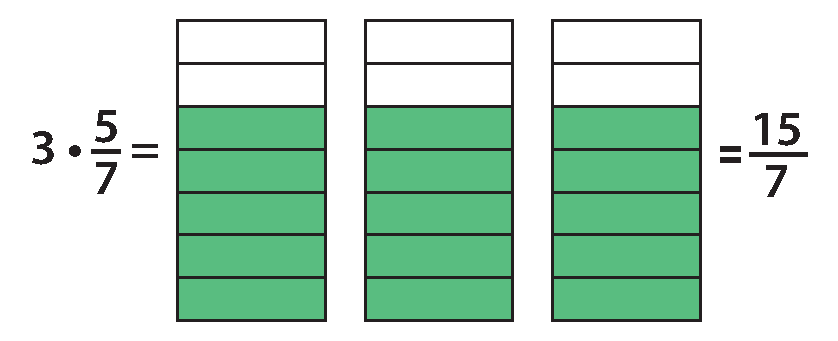
\includegraphics[scale=0.4]{pictures/Kuva3-1-1.pdf}
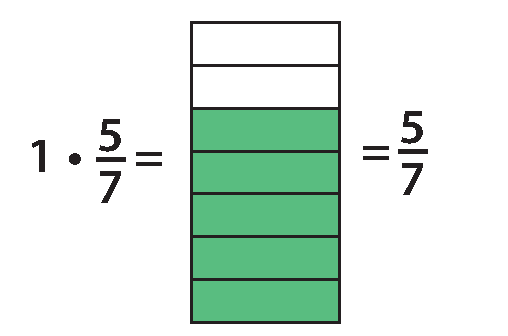
\includegraphics[scale=0.4]{pictures/Kuva3-1-2.pdf}
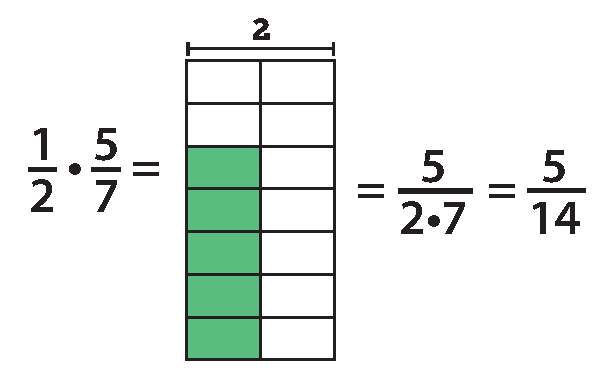
\includegraphics[scale=0.4]{pictures/Kuva3-1-3.pdf}
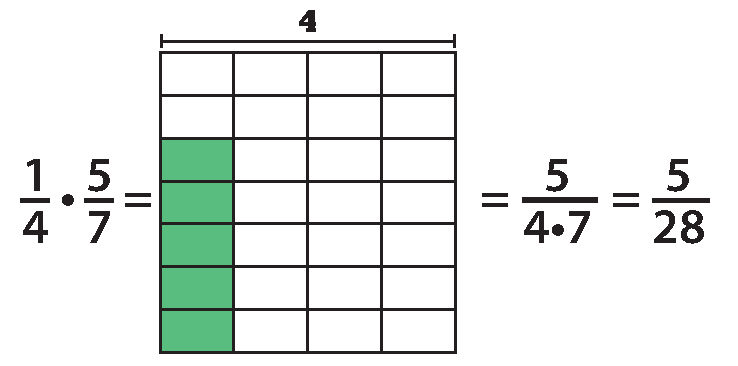
\includegraphics[scale=0.4]{pictures/Kuva3-1-4.pdf}
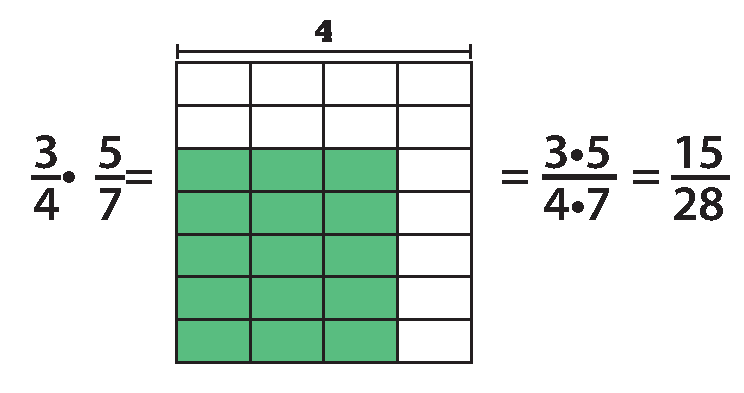
\includegraphics[scale=0.4]{pictures/Kuva3-1-5.pdf}

\begin{esimerkki}
	Luvun $5$ \termi{käänteisluku}{käänteisluku} on $\frac{1}{5}$, koska
	\[
	 5\cdot \frac{1}{5}=1.
	\]
	Vastaavasti luvun $-\frac{2}{3}$ käänteisluku on $-\frac{3}{2}$, koska
	\[
	 -\frac{2}{3}\cdot (-\frac{3}{2})=1.
	\]

\end{esimerkki}
\laatikko{
    Rationaaliluvun $a$ ($a\neq 0$) \termi{käänteisluku}{käänteisluku} on  $\frac{1}{a}$, sillä
    \[
    a\cdot \frac{1}{a} = 1.
    \]
    Vastaavasti rationaaliluvun $\frac{a}{b}$ ($a\neq 0$ ja $b\neq 0$) käänteisluku on $\frac{b}{a}$, sillä
    \[
    \frac{a}{b}\cdot \frac{b}{a} = 1.
    \]    

  %  Murtolukujen $p=\frac{a}{b}$ ja $q=\frac{c}{d}\neq 0$ \termi{osamäärä}{osamäärä} $p : q$ saadaan, kun kerrotaan luku $p$ luvun $q$ käänteisluvulla,
 %   \[
 %\frac{p}{q} = p\cdot q^{-1} = \frac{a}{b}\cdot\Big(\frac{c}{d}\Big)^{-1} = \frac{a}{b}\cdot \frac{d}{c}
 %   = \frac{ad}{bc}.
 %  \]
 }

\begin{esimerkki}
Kuinka lasketaan murtolukujen jakolasku $\frac 3 5 : \frac 2 7$? Jakolaskun määritelmän mukaan osamäärän tulisi olla sellainen luku, joka kerrottuna jakajalla antaa tulokseksi jaettavan. Jos merkitään laskun $\frac 3 5 : \frac 2 7$ vastausta kirjaimella $x$, pitää siis olla $x \cdot \frac 2 7 = \frac 3 5$.  Tätä yhtälöä kutsutaan jakolaskun $\frac 3 5 : \frac 2 7$ \termi{jakoyhtälö}{jakoyhtälöksi.}

Kerrotaan jakoyhtälön molemmat puolet luvun $\frac 2 7$ käänteisluvulla $\frac 7 2$. Koska käänteislukujen tulo on $1$, saadaan
\[
	\text{vasen puoli} = x \cdot \underbrace{\frac 2 7 \cdot \frac 7 2}_{= 1} = x \quad \text{ja} \quad \text{oikea puoli} = \frac 3 5 \cdot \frac 7 2.
\]

Kun yhtälön molemmat puolet kerrotaan samalla luvulla, ovat myös näin saadut luvut yhtä suuria. Siis on saatu
\[
	x = \frac 3 5 \cdot \frac 7 2.
\]
Koska $x$:llä merkittiin alkuperäistä jakolaskua, on nyt onnistuttu muuttamaan jakolasku kertolaskuksi:
\[
	\frac 3 5 : \frac 2 7 = \frac 3 5 \cdot \frac 7 2 = \frac{3 \cdot 7}{5 \cdot 2} = \frac{21}{10} = 2 \frac{1}{10}.
\]
Siis jakolasku laskettiin kertomalla jaettava jakajan käänteisluvulla. Näin toimitaan yleisestikin.
 \end{esimerkki}

\laatikko{
Olkoon $b \neq 0$, $c \neq 0$ ja $d \neq 0$. Murtolukujen osamäärä $\frac a b : \frac c d$ lasketaan kertomalla jaettava jakajan käänteisluvulla:
\[
	\frac a b : \frac c d = \frac a b \cdot \frac d c = \frac{ad}{bc}.
\]
}

Samannimisten murtolukujen vertailu on helppoa: jos $a > 0$, $\frac{b}{a} < \frac{c}{a}$ täsmälleen silloin kun $b < c$. Yleisten murtolukujen
vertailu voidaan tehdä siis laventamalla luvut samannimisiksi:

\laatikko{
Kahta murtolukua voidaan vertailla laventamalla ne samannimisiksi siten, että yhteinen nimittäjä on positiivinen, ja sitten vertaamalla osoittajia.
}
    
    \begin{esimerkki}
        Salamipizza jaetaan kuuteen ja tonnikalapizza neljään yhtä suureen
        siivuun. Vesa saa kaksi siivua salamipizzaa ja yhden siivun tonnikalapizzaa.
        Minttu saa kaksi siivua tonnikalapizzaa. Kumpi saa enemmän pizzaa, jos
        molemmat pizzat ovat saman kokoisia?
        
        \begin{center}        
          
\includegraphics[scale=1.0]{pictures/Kuva3-1-6-pizzat.pdf}
        \end{center}

        \textbf{Ratkaisu.}
        
        Huomataan, että $12 = 3\cdot 4 = 2\cdot 6$. Luvut kannattaa
        pizzan kokonaismäärän laskemista varten laventaa niin, että
        nimittäjänä on luku $12$.
        Vesan saama määrä pizzaa on
        \begin{align*}
           \frac{2}{6} + \frac{1}{4} &= \frac{2\cdot 2}{2\cdot 6} + \frac{3\cdot 1}{3\cdot 4} \\ 
	       							 &= \frac{4}{12}+\frac{3}{12} \\ 
	       							 &= \frac{7}{12}.
        \end{align*}
        
        Mintun saama määrä pizzaa on
        \[
            \frac{2}{4} =
            \frac{3\cdot 2}{3\cdot 4} =
            \frac{6}{12}.
        \]
        Koska $6/12 < 7/12$, Vesa saa enemmän.
    \end{esimerkki}
    
    Kaikki rationaaliluvut voidaan esittää murtolukumuodossa, mutta myös
    kokonaisluvut voidaan esittää murtolukuina asettamalla murtoluvun
    nimittäjäksi yksi. Tätä voidaan käyttää, kun lasketaan yhteen
    kokonaislukuja ja murtolukuja.
    
    \begin{esimerkki}
        Laske
        \[
            2 + \frac{1}{3}.
        \]
        
        \textbf{Ratkaisu.}
        
%        Kirjoitetaan aluksi
%        \[
%            2=\frac{2}{1}.
%        \]
		Kirjoitetaan lausekkeen kokonaisluku $2$ murtolukuna, jonka
		jälkeen voidaan murtoluvut voidaan laventaa samannimisiksi
		ja laskea yhteen:
        \begin{align*}
           2 + \frac{1}{3} &= \frac{2}{1} + \frac{1}{3}  \\ 
	       				   &= \frac{3 \cdot 2}{3 \cdot 1} + \frac{1}{3} \\ 
	       				   &= \frac{6+1}{3} \\ 
	       				   &= \frac{7}{3}.
        \end{align*}
    \end{esimerkki}
